\section{Desarrollo}

\subsection{Referencias}
Los elementos del listado de referencias deben escribirse en el archivo \verb!Referencias.bib! siguiendo el formato allí establecido. Para citar una referencia en el documento se utiliza el comando \verb!\cite{X}!, donde \verb!X! es el nombre que se le da a cada elemento de las referencias. Por ejemplo, en el listado provisto hay dos elementos cuyos nombres son \verb!ref1! y \verb!ref2!. Al citar ambas referencias de forma independiente quedaría \cite{ref1} y \cite{ref2}. También se pueden citar ambas juntas así \cite{ref1, ref2}.

\subsection{Listas de elementos}
Se pueden crear listas de elementos mediante el ambiente \verb!itemize!. El ambiente se abre con \verb!\begin{itemize}!, los elementos se agregan mediante el comando \verb!\item! y el ambiente se cierra con \verb!\end{itemize}!. A continuación un ejemplo:

\begin{itemize}
    \item Primer elemento
    \item Segundo elemento
    \item Tercer elemento
    \item Cuarto elemento
\end{itemize}

\subsection{Acrónimos y siglas}
Este formato no contempla una nomenclatura ni uso automático de acrónimos o siglas. La primera vez que se usa una abreviación en particula se escribe definición extensa seguida por la abreviación entre paréntesis. Las siguientes veces solo se usa la abreviación. Por ejemplo, se definen los conceptos emisiones acústicas (EA) y red neuronal convolucional (RNC). Si los volvemos a utilizar nuevamente, solo se usan las abreviaciones EA y RNC.

\subsection{Ecuaciones y símbolos matemáticos}
Se pueden crear ecuaciones numeradas mediante el ambiente \verb!equation!. El ambiente se abre con \verb!\begin{equation}!, se ingresa la ecuación deseada y el ambiente se cierra con \verb!\end{equation}!. A continuación un ejemplo:
\begin{equation}\label{eq:signature}
    x(t) = x_{r}(t) + \frac{s(t)}{2\pi} - \int_{a}^{b} h(r) dr
\end{equation}
Esta ecuación numerada se puede referenciar en el texto mediante el comando \verb!\ref{X}!, donde \verb!X! es la etiqueta o \textit{label} que se le dio a la ecuación dentro del ambiente. En este caso corresponde a la Ec.~\ref{eq:signature}.

Para insertar ecuaciones o símbolos matemáticos dentro de un párrafo se usa \verb!$X$!, donde \verb!X! es lo que se desea escribir. Por ejemplo, se escribe la ecuación de una recta $y = mx + b$ dentro del párrafo. También se pueden escribir símbolos matemáticos latinos en cursiva como $x, r^{2}, c_{p}$ o griegos como $\alpha, \pi, \Delta$.

\subsection{Figuras}
\subsubsection{Figuras simples}
Las figuras se insertan en el ambiente \verb!figure!. El ambiente se abre con \verb!\begin{figure}!, se añade la ruta relativa a la figura con el comando \verb!\includegraphics! y el ambiente se cierra con \verb!\end{figure}!. La figura puede tener diferentes extensiones, entre ellas .png, .jpg y .pdf. A continuación un ejemplo:

\begin{figure}[h]
    \centering    
    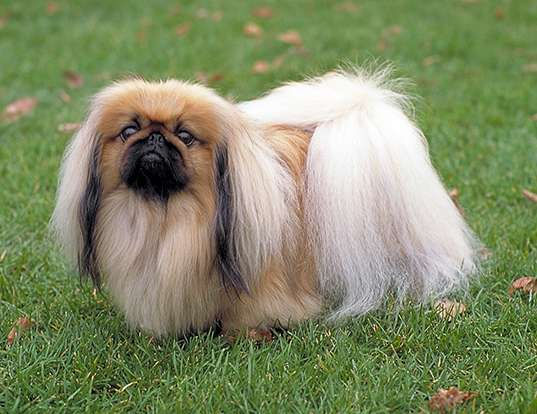
\includegraphics[width=0.5\textwidth]{F-Pequines.jpg} 
    \caption{Perro de raza pequinés}
    \label{fig:F-Pequines}
\end{figure}

El ambiente ofrece diferentes opciones para ajustar la alineación, posición y tamaño. El título bajo la figura se cambia mediante el comando \verb!\caption!. La referencia dentro del texto se hace igual que las ecuaciones. Es decir, se le da a la figura una etiqueta con el comando \verb!\label! y luego se referencia con el comando \verb!\ref!. En este caso resulta Fig.~\ref{fig:F-Pequines}.

\subsubsection{Figuras múltiples}
Es posible usar estructuras más complejas para añadir figuras múltiples como la Fig.~\ref{fig:Dos-Perros}.

\begin{figure*}[h]
    \centering
    \begin{subfigure}[t]{0.4\textwidth}
        \centering{%
        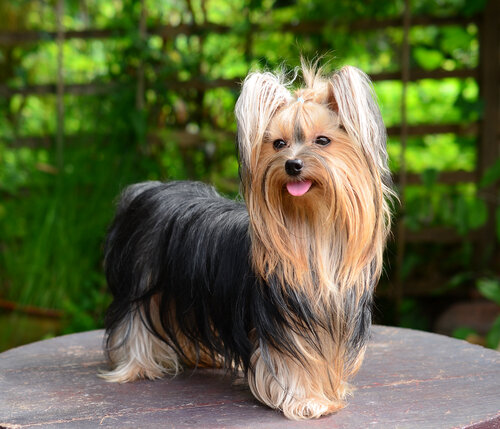
\includegraphics[width=\textwidth]{F-Yorkshire.jpg}
        }%
        \subcaption{Yorkshire\label{fig:F-Yorkshire}}
        \end{subfigure}
    \begin{subfigure}[t]{0.3435\textwidth}
        \centering{%
        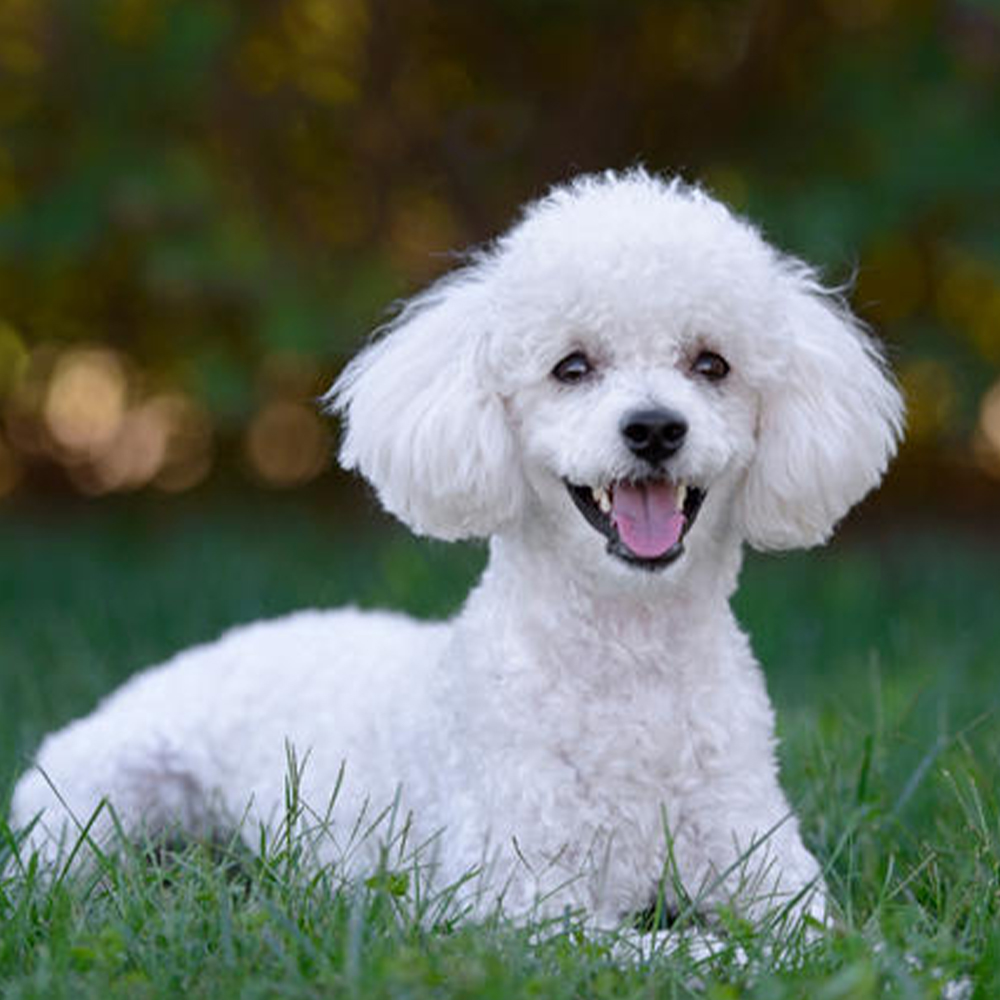
\includegraphics[width=\textwidth]{F-Poodle.jpg}
        }%
        \subcaption{Poodle\label{fig:F-Poodle}}
    \end{subfigure}
    \caption{Perros de diferente raza.}\label{fig:Dos-Perros}
\end{figure*}

En este caso, un perro yorkshire se muestra en la Fig.~\ref{fig:F-Yorkshire}, mientras que un perro poodle se muestra en la Fig.~\ref{fig:F-Poodle}

\subsection{Tablas}
\subsubsection{Tablas simples}
Las tablas se insertan en el ambiente \verb!table! combinado con \verb!tabular!. Al llamar al ambiente \verb!tabular! se deben especificar la cantidad de columnas de la tabla escribiendo una \textbf{c} por cada columna con alineación centrada. Luego, los datos se añaden por cada fila separados por el símbolo \& y terminando la fila con doble backslash. Los comandos del tipo x-\verb!rule! son para añadir líneas horizontales. El comando \verb!label! es para darle el título a la tabla. A continuación un ejemplo:

\begin{table}[h]
	\centering
	\caption{CNN architecture}
	\label{tab:CNNArchitecture}
	\begin{tabular}{cccc}
		\toprule
		Layer & Kernel size & Number of kernels & Feature map size \\
		\midrule
		Input & - & - & 128x128 \\
		Convolution 1 & 5x5 & 64 & 124x124 \\
		Pooling 1 & 2x2 & 64 & 62x62 \\
		Convolution 2 & 5x5 & 32 & 62x62 \\
		Pooling 2 & 2x2 & 32 & 31x31 \\
		Fully connected & 1x1 & 512 & 512 \\
		Softmax & - & - & 5 \\
		\bottomrule
	\end{tabular}
\end{table}

La referencia de las tablas en el texto se realiza de la misma manera que para ecuaciones y figuras. En este caso tenemos la Tabla~\ref{tab:CNNArchitecture}.


\subsubsection{Tablas personalizadas}
Se pueden crear tablas personalizadas combinando filas y columnas mediante los comandos \verb!\multicolumn! y \verb!\multirow!. La Tabla~\ref{tab:norm-type} muestra un ejemplo de esto

\begin{table}[h]
	\centering
	\caption{Accuracy for different signal durations considering the three types of image normalization}
	\label{tab:norm-type}
	\begin{tabular}{cccc}
		\toprule
		Signal duration & Normalization & Average \% & Std. deviation \% \\
		\midrule
		\multirow{3}{*}{0.6 s} & Global & 80 & 12 \\
		 & Local & 78 & 12 \\
		 & Signal & 50 & 36 \\
             \midrule
		\multirow{3}{*}{1.0 s} & Global & \multicolumn{2}{c}{Not considered} \\
		 & Local & 88 & 6 \\
		 & Signal & 90 & 76 \\
             \midrule
		\multirow{3}{*}{10 rev} & Global & \multicolumn{2}{c}{Not considered} \\
		 & Local & 59 & 49 \\
		 & Signal & \multicolumn{2}{c}{Not considered} \\
		\bottomrule
	\end{tabular}
\end{table}


